Plump \cite{plump2018modular} later proposed a modular critical pair-based strategy for left-injective DPO hypergraph rewriting with monic matches. 
Our method complements this: while modularity reduces global complexity, each subsystem requires individual termination proofs. 

We brively recall the basic definitions of hypergraphs and show that a graph is a hypergraph.

 For a more comprehensive introduction to DPO hypergraph rewriting, we refer the reader to \cite{plump2018modular}. 

\begin{definition}
    A signature $\Sigma = \langle \Sigma_V, \Sigma_E, \text{Type} \rangle$ consists of 
    \begin{itemize}
        \item a set $\Sigma_V$ of node labels,
        \item a set $\Sigma_E$ of hyperedge labels, and
        \item a function $\text{Type}$ assigning to each $l \in \Sigma_E$ a set of strings $\text{Type}(l) \subseteq \Sigma_V^*$.
    \end{itemize}
\end{definition}
Unless stated otherwise, we denote by $\Sigma$ an arbitrary but fixed signature over which all hypergraphs are labelled.

\begin{remark}
    The extension $f^* : A^* \to B^*$ of a function $f : A \to B$ maps the empty string to itself and $a_1 \ldots a_n$ to $f(a_1) \ldots f(a_n)$.
\end{remark}
\begin{definition}
    A hypergraph over $\Sigma$ is a system $G = \langle V_G, E_G, \text{mark}_G, \text{lab}_G, \text{att}_G \rangle$ consisting of 
    \begin{itemize}
        \item a finite set $V_G$ of nodes,
        \item a finite set $E_G$ of hyperedges,
        \item two labelling functions $\text{mark}_G : V_G \to \Sigma_V$ and $\text{lab}_G : E_G \to \Sigma_E$, and
        \item an attachment function $\text{att}_G : E_G \to V_G^*$ such that $\text{mark}_G^*(\text{att}_G(e)) \in \text{Type}(\text{lab}_G(e))$ for each hyperedge $e$.
    \end{itemize} 
\end{definition} 

\begin{definition}[Sequential independence]
    \todo{rewrite}
   Direct derivations $G \Rightarrow_{r_1} H \Rightarrow_{r_2} M$ as in Figure 4 are sequentially independent if there are morphisms $R_1 \to D_2$ and $L_2 \to D_1$ such that the following holds.
    \begin{itemize}
        \item Commutativity: $R_1 \to D_2 \to H = R_1 \to H$ and $L_2 \to D_1 \to H = L_2 \to H$.
        \item Injectivity: $R_1 \to D_2 \to M$ is injective.
    \end{itemize}
    
    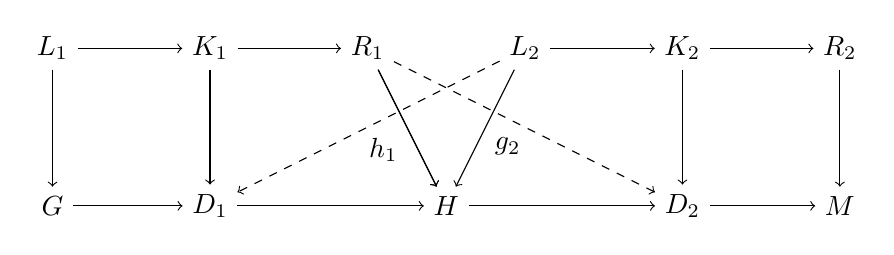
\begin{tikzpicture} 
        % Define nodes
        \node (L1) at (0,2) {$L_1$};
        \node (K1) at (2,2) {$K_1$};
        \node (R1) at (4,2) {$R_1$};
        \node (L2) at (6,2) {$L_2$};
        \node (K2) at (8,2) {$K_2$};
        \node (R2) at (10,2) {$R_2$};
        \node (G) at (0,0) {$G$};
        \node (T) at (5,0) {$H$};
        \node (M) at (10,0) {$M$};
        \node (D1) at (2,0) {$D_1$};
        \node (D2) at (8,0) {$D_2$};
      
        % Draw arrows
        % Top row
        \draw[->] (L1) -- node[above] {} (K1);
        \draw[->] (K1) -- node[above] {} (R1);
        \draw[->] (L2) -- node[above] {} (K2);
        \draw[->] (K2) -- node[above] {} (R2);
      
        % Vertical arrows
        \draw[->] (L1) -- node[left] {} (G);
        \draw[->] (R1) -- node[right] {} (T);
        \draw[->] (R2) -- node[right] {} (M);
        \draw[->] (K1) -- node[right] {} (D1);
        \draw[->] (K2) -- node[right] {} (D2);
      
        % Bottom row
        \draw[->] (G) -- node[below] {} (D1);
        \draw[->] (D1) -- node[below] {} (T);
        \draw[->] (T) -- node[below] {} (D2);
        \draw[->] (D2) -- node[below] {} (M);

        \draw[->,dashed] (R1) -- node[below] {} (D2);
        \draw[->,dashed] (L2) -- node[below] {} (D1);
      
        % Diagonal arrows
        \draw[->] (R1) -- node[below left] {$h_1$} (T);
        \draw[->] (L2) -- node[below right] {$g_2$} (T);
      \end{tikzpicture}
\end{definition}

\begin{definition}[Sequential critical pair]
    Let $r_i \colon \langle L_i \leftarrow K_i \rightarrow R_i \rangle$ be rules, for $i = 1, 2$. A pair of direct derivations $G \Rightarrow_{r_1} H \Rightarrow_{r_2} M$ as depicted below is a sequential critical pair if the following holds.
    \begin{itemize}
        \item Minimality:$H = h_1(R_1) \cup g_2(L_2)$.
        \item Conflict: The steps are not sequentially independent.
    \end{itemize}
    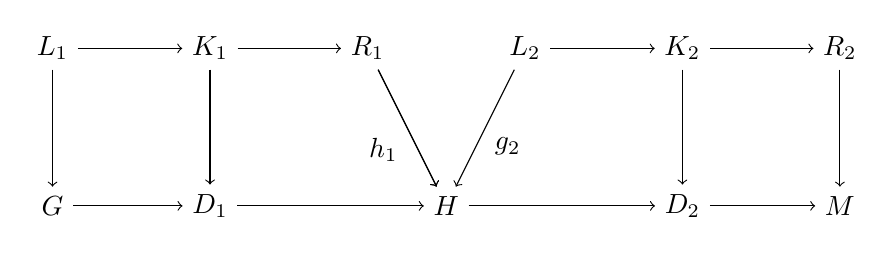
\begin{tikzpicture} 
        % Define nodes
        \node (L1) at (0,2) {$L_1$};
        \node (K1) at (2,2) {$K_1$};
        \node (R1) at (4,2) {$R_1$};
        \node (L2) at (6,2) {$L_2$};
        \node (K2) at (8,2) {$K_2$};
        \node (R2) at (10,2) {$R_2$};
        \node (G) at (0,0) {$G$};
        \node (T) at (5,0) {$H$};
        \node (M) at (10,0) {$M$};
        \node (D1) at (2,0) {$D_1$};
        \node (D2) at (8,0) {$D_2$};
      
        % Draw arrows
        % Top row
        \draw[->] (L1) -- node[above] {} (K1);
        \draw[->] (K1) -- node[above] {} (R1);
        \draw[->] (L2) -- node[above] {} (K2);
        \draw[->] (K2) -- node[above] {} (R2);
      
        % Vertical arrows
        \draw[->] (L1) -- node[left] {} (G);
        \draw[->] (R1) -- node[right] {} (T);
        \draw[->] (R2) -- node[right] {} (M);
        \draw[->] (K1) -- node[right] {} (D1);
        \draw[->] (K2) -- node[right] {} (D2);
      
        % Bottom row
        \draw[->] (G) -- node[below] {} (D1);
        \draw[->] (D1) -- node[below] {} (T);
        \draw[->] (T) -- node[below] {} (D2);
        \draw[->] (D2) -- node[below] {} (M);

        % \draw[->,dashed] (R1) -- node[below] {} (D2);
        % \draw[->,dashed] (L2) -- node[below] {} (D1);
      
        % Diagonal arrows
        \draw[->] (R1) -- node[below left] {$h_1$} (T);
        \draw[->] (L2) -- node[below right] {$g_2$} (T);
      \end{tikzpicture}
\end{definition}

\begin{theorem}
    \todo{rewrite}
    Let $\langle \Sigma, \mathcal{R} \rangle$ and $\langle \Sigma, \mathcal{S} \rangle$ be terminating hypergraph transformation systems. If there are no sequential critical pairs of shape $S \Rightarrow_{\mathcal{R}} T \Rightarrow_{\mathcal{S}} U$, then the combined system $\langle \Sigma, \mathcal{R} \cup \mathcal{S} \rangle$ is terminating.
\end{theorem}
